\documentclass{standalone}
\usepackage{tikz}
\usetikzlibrary{arrows.meta, positioning}

\begin{document}

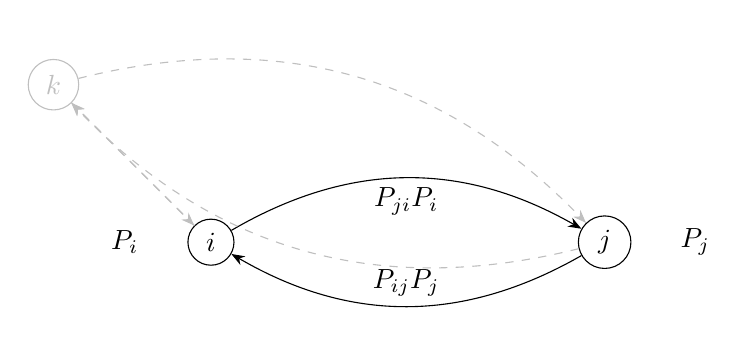
\begin{tikzpicture}[node distance=3cm, >=Stealth]
    % Nodes
    \node[draw, circle] (i) at (0,0) {$i$};
    \node[draw, circle] (j) at (5,0) {$j$};
    \node[draw, circle, lightgray] (k) at (-2,2) {$k$};
    
    % Arrows with text labels
    \draw[->] (j) to[bend left] node[midway, above] {$P_{ij} P_j$} (i);
    \draw[->] (i) to[bend left] node[midway, below] {$P_{ji} P_i$} (j);
    
    % Light gray dashed connections to other states
    \draw[->, lightgray, dashed] (k) to (i);
    \draw[->, lightgray, dashed] (i) to (k);
    \draw[->, lightgray, dashed] (k) to[bend left] (j);
    \draw[->, lightgray, dashed] (j) to[bend left] (k);
    
    % Labels for probabilities
    \node[draw=none, left=0.5cm of i] {$P_i$};
    \node[draw=none, right=0.5cm of j] {$P_j$};
\end{tikzpicture}

%\caption{Illustration of Detailed Balance in a Markov Chain}
%\label{fig:detailed_balance}

\end{document}
